\section{Motivation}
\label{s:motivation}

\begin{figure*}[t]
  \begin{center}
    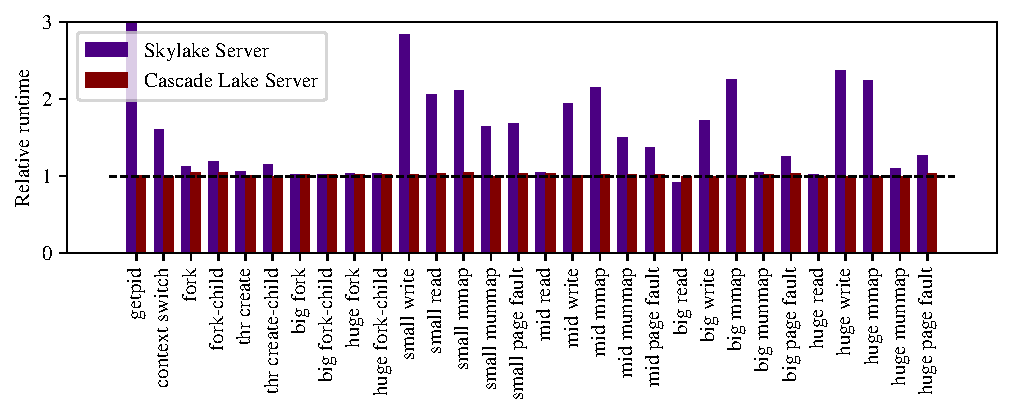
\includegraphics[width=\textwidth]{results/bhw2_bhw3_overhead}
  \end{center}
\vspace{-\baselineskip}
\caption{Linux slowdown due to mitigations on \bench, for two generations of Intel CPUs: Broadwell and Cascade Lake.}
\label{fig:linuxslowdown}
\end{figure*}

% \begin{figure*}[t]
%   \begin{center}
%     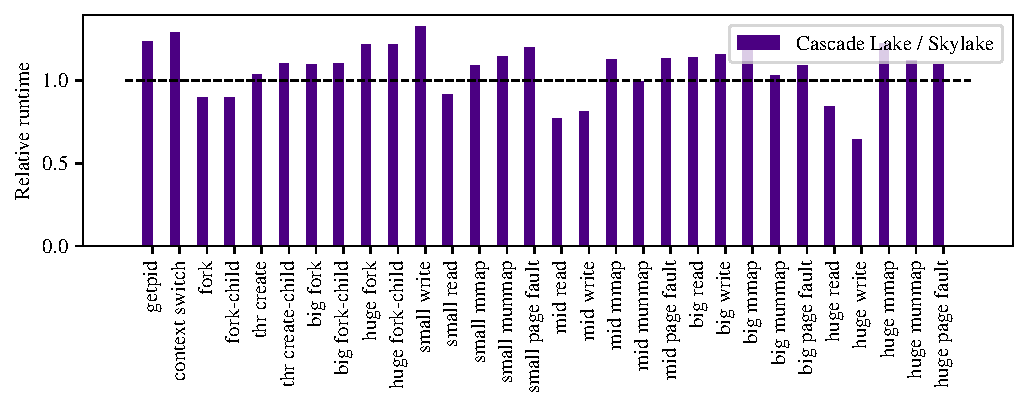
\includegraphics{results/cascade_lake_regression}
%   \end{center}
% \vspace{-\baselineskip}
% \caption{Performance regression on the newer Cascade Lake CPU, compared to the older Broadwell CPU,
%   for \bench on Linux, with all software-controllable mitigations disabled.}
% \label{fig:regression}
% \end{figure*}

Transient execution mitigations harm kernel performance in two
ways. First, they place overhead on code execution by disabling
speculation, like how the Linux Kernel uses retpolines to
mitigate Spectre V2. That involves replacing each indirect branch in the kernel with a
sequence of instructions that prevent the CPU from performing branch
target speculation~\cite{intel:retpoline}. Second, mitigations
increase the privilege mode switching cost incurred during each system
call: upon entry into the kernel, they either flush microarchitectural
state or reconfigure protection mechanisms.  For example,
KPTI~\cite{gruss:kaiser,linux:kpti} switches to a separate page table
before executing kernel code to prevent Meltdown
attacks~\cite{lipp:meltdown}.  As described before, workloads
that are system call intensive (e.g., web servers, version control
systems, etc.) are impacted by this type of overhead, while compute-intensive
workloads see little performance impact.

Collectively, these and other mitigations can result in large
slowdowns. 
To better understand this problem, we revisit the 
\bench~\cite{lebench} microbenchmark suite from earlier which
consists of system calls
that impact application
performance the most, this time examining individual system calls instead of only the geometric mean over all of them.
We evaluate the Linux kernel (version 5.6.13),
comparing two configurations: one where all mitigations are disabled
and one where all are enabled. \autoref{fig:linuxslowdown} shows
the relative slowdown between the two configurations for 13 kernel
operations of \bench that don't involve networking (i.e., without
\texttt{send}, \texttt{recv}, \texttt{epoll}).  There are two sets of
bars, representing two generations of Intel CPUs: the older Broadwell,
and the newer Cascade Lake.  On the older Broadwell CPUs,
system calls that perform the least kernel work are impacted the most
(e.g., \texttt{getpid()}), but a wide range of operations are impacted
significantly (25\%-100\% slowdowns). These observations are similar
to what we saw in \autoref{sec:benchmarks:lebench} and to the observations made by Ren et. al.~\cite{lebench}.

% The newer Cascade Lake CPUs exhibit lower relative overheads, partly
% because the processors include hardware mitigations for some of the
% transient execution vulnerabilities.  However, these lower overheads
% are also in part due to the newer Cascade Lake CPUs being \emph{slower}
% in the baseline case when software-controllable mitigations are disabled.
% Figure~\ref{fig:regression} shows the performance of the microbenchmark
% on Cascade Lake (Intel Xeon Silver 4210R) relative to the earlier
% Broadwell CPU (Intel Xeon E5-2640 v4).  Our experiment uses CPUs
% with identical clocks (2.4~GHz), and nearly identical other hardware
% (Dell PowerEdge T430 vs. T440), which allows the comparison to be
% meaningful.  The results demonstrate that, although the new CPU is
% faster at some microbenchmarks, it is slower for many others: e.g.,
% context-switching is about 20\% slower.  Although it is impossible for us to
% separate slowdowns due to mitigations from speedups due to architectural
% improvements, the results suggest that the overheads of mitigations implemented
% in hardware (e.g., for Meltdown, L1TF, or MDS) could still be significant.
% \footnote{One indication that this regression may be related to hardware
%   mitigations is that measured branch mispredictions are around 40\% higher on
%   LEBench.}

%\fk{table 11 in ~\cite{sok:transient} claims the overhead of KPTI is
%  small, < 3\%}

%Avoiding these overheads normally requires making compromises to
%security; disabling any one of them would leave the kernel vulnerable
%to a transient execution attack.
%Our goal, instead, is to apply these
%mitigations only when they are needed to protect data that should be
%kept secret from the running process.
%We now describe our approach to
%restructuring the kernel so it can achieve this goal.
